Conforme dito anteriormente o trabalho busca o desenvolvimento do design do circuito integrado de um DPD, a partir de um modelo validado em software, e em hardware, no caso, FPGA. Para isso esse projeto foi divido em 4 etapas principais:

\begin{itemize}
    \item Estudo DPD;
    \item Implementação em software;
    \item Implementação em FPGA;
    \item Design e validação do circuito integrado.
\end{itemize}

\section{Estudo dos DPDs}
A etapa consistia so estudo dos DPDs que foi apresentado no capitulo \ref{chap:revi}, onde e feito todo o estudo e levantamento sobre os tipos de modelagem do DPDs. 

\section{Implementação em software}
Nesta etapa é feito a implementação propriamente dita do modelo do DPD em software, para isso foi utilizado a linguagem de programação python que é uma linguagem de programação amigavel, bastante difundida na comunidade academica e prática de ser utilizada.
Para fazer essa modelagem foram coletados sinais de entrada e de saída de um amplificador de potência classe AB, que utiliza um HEMT fabricado em tecnologia GaN. O amplificador foi excitado por um sinal portadora de frequência de 900 MHz e modulado por um sinal de envelope WCDMA 3GPP com cerca de 3,84 MHz de largura de banda. Os dados de entrada e saída do amplificador de potência foram medidos usando um VSA Rohde \& Schwarz FSQ com uma taxa de amostragem de 61,44 MHz, disponível em \cite{Bonfim2016}.
Para tal 

\section{Implementação em FPGA}


\section{Design e validação}
Finalmente, na última etapa, realiza-se o processo de concepção do circuito integrado do DPD como um circuito dedicado integrado na tecnologia BiCMOS 130 nm 8HP, utilizando as ferramentas do Cadence.
O fluxo de projeto VLSI  para design de um circuito integrado de aplicação específica, inclui a descrição do circuito em VHDL, síntese lógica utilizando as células padrão da tecnologia, place and route e simulações comportamentais e temporais. O diagrama do fluxo VLSI pode ser ilustrado pela figura \ref{fig:CMOS2010}.

\begin{figure}[ht!]
    \centering
    \captionsetup{justification=centering}
    \caption*{Fonte: \cite{CMOS2010}}
    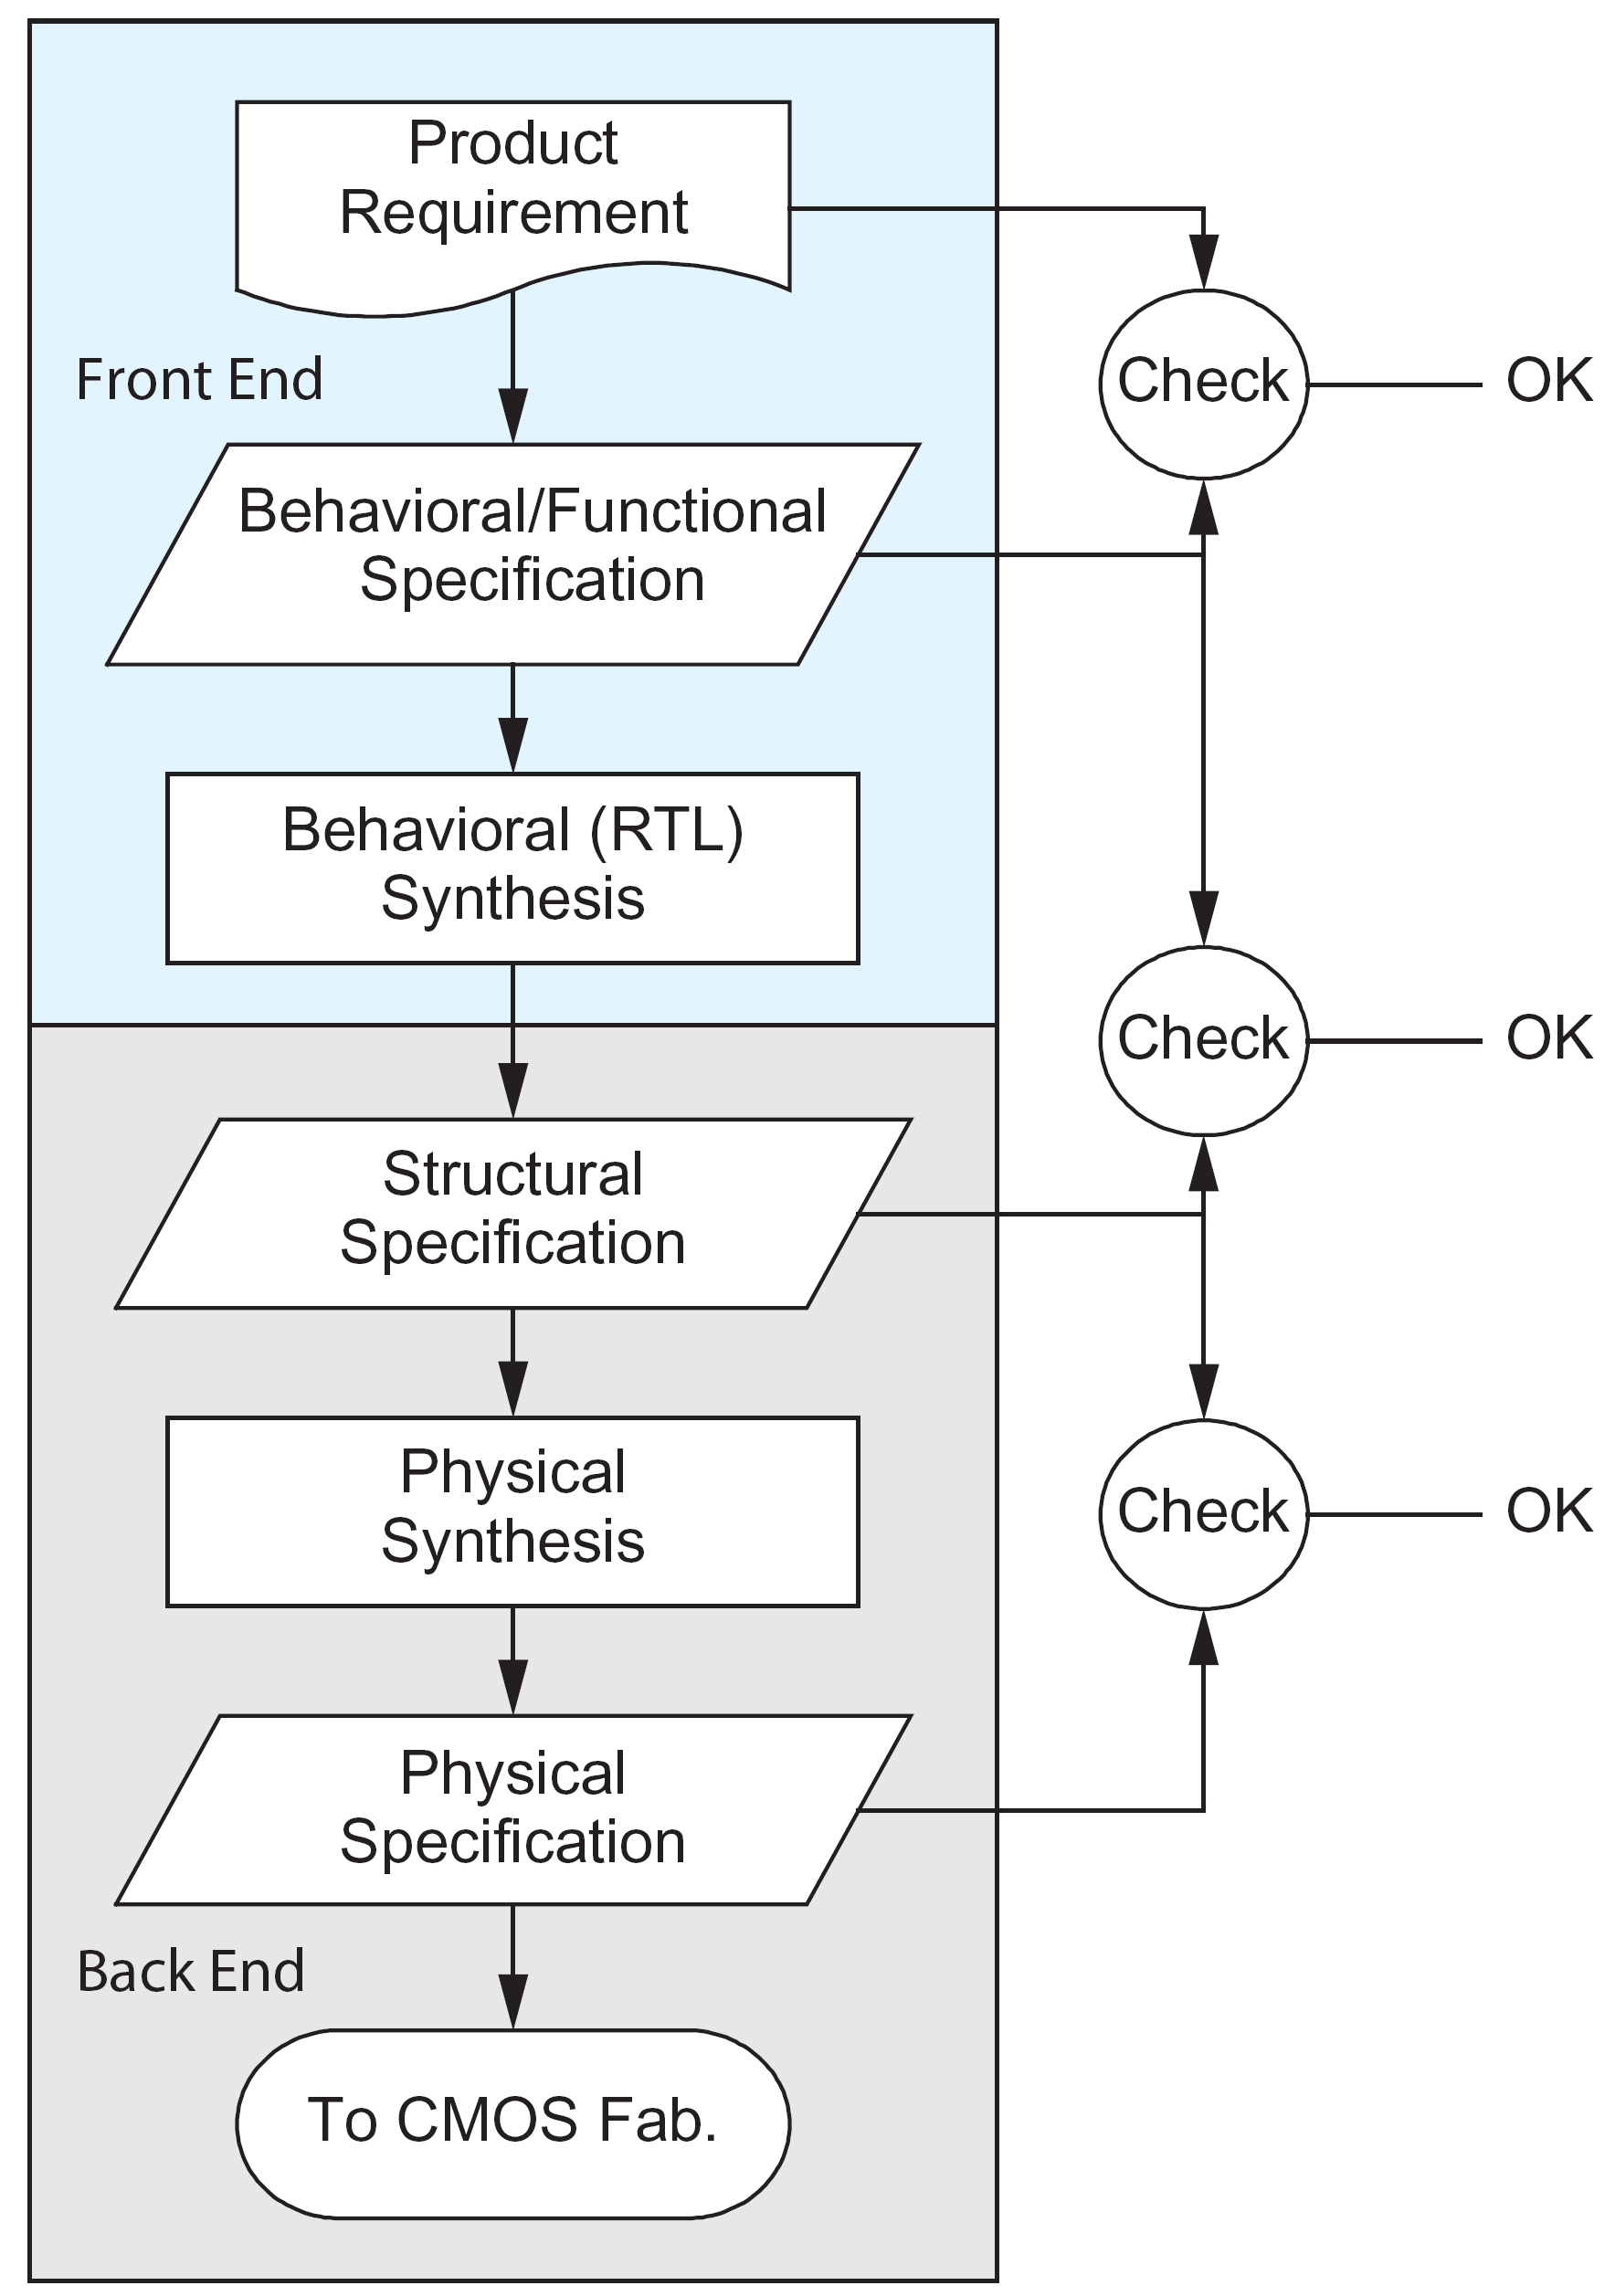
\includegraphics[width=0.5\textwidth]{fluxovlsi.png}
    \caption{Fluxo de projeto VLSI}
    \label{fig:CMOS2010}
\end{figure}

No processo de desenvolvimento do circuito, várias etapas são executadas. Primeiro, há a simulação comportamental para verificar se o circuito VHDL atende às expectativas, utilizando um testbench em VHDL e a ferramenta Cadence NCLaunch. Em seguida, ocorre a síntese lógica, onde a partir do modelo comportamental, utiliza-se a ferramenta Genus para criar um modelo RTL com células padrão de tecnologia específica, considerando restrições de área, frequência e consumo de energia. A síntese gera dois arquivos: um com componentes e conexões, em Verilog, e outro com informações de atraso no formato SDF. A simulação pós-síntese é realizada para validar o netlist gerado, usando o mesmo testbench da simulação comportamental. Em seguida, na etapa de PAR, o layout é criado posicionando as células e realizando as conexões entre essas células, utilizando a ferramenta Innovus. Por fim, na simulação pós-PAR, o circuito é simulado considerando as resistências e capacitâncias parasitas. Cada etapa é fundamental para garantir o correto funcionamento do circuito.